% Sequence diagram: login (Figure 4.8)
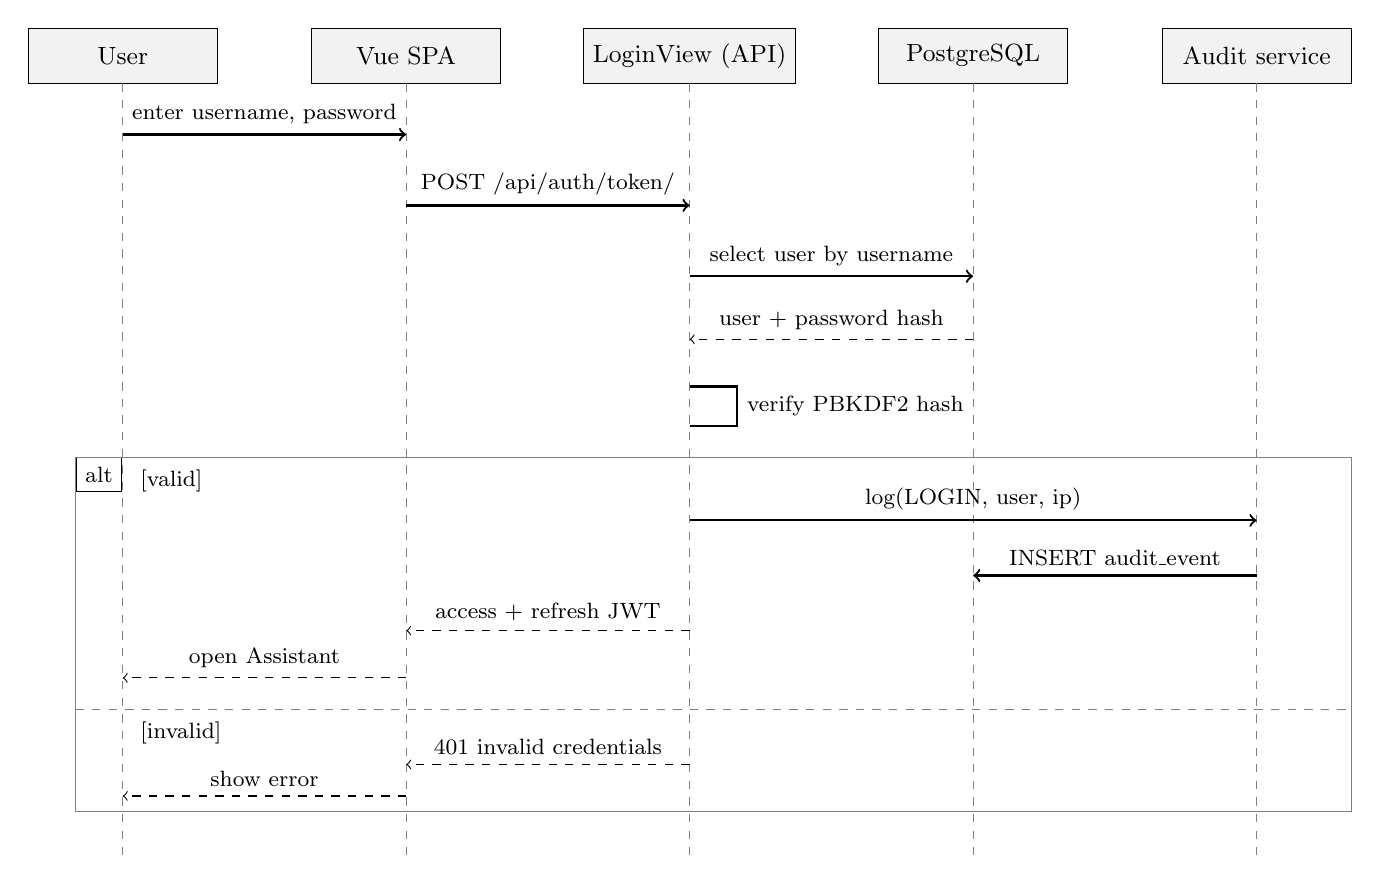
\begin{tikzpicture}[
  ll/.style={draw,fill=gray!10,font=\small,minimum width=24mm,minimum height=7mm,align=center},
  msg/.style={->,thick,font=\footnotesize},
  ret/.style={->,dashed,font=\footnotesize}]
\foreach \x/\n/\t in {0/u/User, 3.6/s/Vue SPA, 7.2/a/LoginView (API), 10.8/d/PostgreSQL, 14.4/l/Audit service}
  {\node[ll] (\n) at (\x,0) {\t}; \draw[dashed,gray] (\x,-0.35) -- (\x,-10.2);}
\def\smsg#1#2#3#4{\draw[msg] (#1,#3) -- node[above,font=\footnotesize]{#4} (#2,#3);}
\def\sret#1#2#3#4{\draw[ret] (#1,#3) -- node[above,font=\footnotesize]{#4} (#2,#3);}
\smsg{0}{3.6}{-1.0}{enter username, password}
\smsg{3.6}{7.2}{-1.9}{POST /api/auth/token/}
\smsg{7.2}{10.8}{-2.8}{select user by username}
\sret{10.8}{7.2}{-3.6}{user + password hash}
\draw[thick] (7.2,-4.2) -- ++(0.6,0) -- ++(0,-0.5) node[right,font=\footnotesize,align=left,midway]{verify PBKDF2 hash} -- ++(-0.6,0);
\node[draw,font=\footnotesize,anchor=north west,fill=white] at (-0.6,-5.1) {alt};
\draw[gray] (-0.6,-5.1) rectangle (15.6,-9.6);
\draw[gray,dashed] (-0.6,-8.3) -- (15.6,-8.3);
\node[font=\footnotesize,anchor=west] at (0.1,-5.4) {[valid]};
\smsg{7.2}{14.4}{-5.9}{log(LOGIN, user, ip)}
\smsg{14.4}{10.8}{-6.6}{INSERT audit\_event}
\sret{7.2}{3.6}{-7.3}{access + refresh JWT}
\sret{3.6}{0}{-7.9}{open Assistant}
\node[font=\footnotesize,anchor=west] at (0.1,-8.6) {[invalid]};
\sret{7.2}{3.6}{-9.0}{401 invalid credentials}
\sret{3.6}{0}{-9.4}{show error}
\end{tikzpicture}
